\begin{figure}[htb]
\centering
\begin{tikzpicture}
\scaling{5};
\point{a}{0}{0};
%\point{b}{.5}{0};
\point{c}{1}{0};
\point{d}{2}{.5};
\point{e}{2}{1};
\point{f}{1}{1};
\beam{2}{a}{c}[0][1];
\beam{2}{c}{d}[1][1];
\beam{2}{d}{e}[1][1];
\beam{2}{e}{f}[1][1];
\beam{2}{f}{c}[1][1];
\dimensioning{1}{a}{c}{-1.5}[$l$];
\dimensioning{1}{c}{e}{-1.5}[$l$];
\dimensioning{2}{d}{e}{11.5}[$l/2$];
\dimensioning{2}{c}{d}{11.5}[$l/2$];
%disegno assi
%   \begin{scope}[color=red]
%       \load{1}{a}[180][1][-1];
%       \load{1}{a}[-90][1][-1];
%       \load{1}{c}[180][1][-1];
%       \load{1}{c}[-90][1][-1];
%       \load{1}{d}[180][1][-1];
%       \load{1}{d}[-90][1][-1];
%   \end{scope}
%nomi aste
\notation{4}{a}{c}[$1$];
\notation{4}{c}{d}[$5$];
\notation{4}{d}{e}[$4$];
\notation{4}{f}{e}[$3$];
\notation{4}{c}{f}[$2$];
%nomi punti
\notation{6}{a}{1};
\notation{6}{c}{2};
\notation{6}{f}{3};
\notation{6}{e}{4};
\notation{6}{d}{5};
\end{tikzpicture}
\caption{Indicazione dei nomi dei nodi e delle aste usati nei calcoli successivi}
\label{fig:StrutturaConNomenclatura}
\end{figure}